\documentclass{article}
%\usepackage[english]{babel}%
\usepackage{graphicx}
\usepackage{tabulary}
\usepackage{tabularx}
\usepackage[normalem]{ulem}
\usepackage{cancel}
\usepackage{tikz} 
\usepackage{pdflscape}
\usepackage{colortbl}
\usepackage{lastpage}
\usepackage{multirow}
\usepackage{enumerate}
\usepackage{color,soul}
\usepackage{pdflscape}
\usepackage{hyperref}
%\usepackage[table]{xcolor}
\usepackage{rotating}
\usepackage{amsmath}
\usepackage{fixltx2e}
\usepackage{framed}
\usepackage{mdframed}
\usepackage[T1]{fontenc}
\usepackage[utf8]{inputenc}
\usepackage{textcomp}
\usepackage{siunitx}
\usepackage{ifthen}
\usepackage{fancyhdr}
\usepackage{gensymb}
 \usepackage{newunicodechar}
\usepackage[document]{ragged2e}
\usepackage[margin=1in,top=1.2in,headheight=57pt,headsep=0.1in]
{geometry}
\usepackage{ifthen}
\usepackage{fancyhdr}
\everymath{\displaystyle}
\usepackage[document]{ragged2e}
\usepackage{fancyhdr}
\everymath{\displaystyle}
%\usepackage[table,xcdraw]{xcolor}
\usetikzlibrary{calc}
\usetikzlibrary{arrows}
\linespread{2}%controls the spacing between lines. Bigger fractions means crowded lines%
%\pagestyle{fancy}
%\usepackage[margin=1 in, top=1in, includefoot]{geometry}
%\everymath{\displaystyle}
\linespread{1.3}%controls the spacing between lines. Bigger fractions means crowded lines%
%\pagestyle{fancy}
\pagestyle{fancy}
\setlength{\headheight}{56.2pt}



\begin{document}

Aside from the Pacific Ocean, this beautiful region of sunny Southern California (SoCal) is not really known for our plethora of abundant water supplies.  The majority of California's 40 million people live in SoCal, and it continues to grow!   So how do we find enough water supplies to meet our water demand?\\
\vspace{1cm}
SoCal has local water supplies from groundwater, surface water, and desalinated water.  However, SoCal continues to import water from outside the SoCal region.  Imported water is water from one hydrologic region that is transferred to another hydrologic region.\\

\vspace{1cm}
The two primary sources of imported water to SoCal are the California State Water Project (SWP) and Colorado River Aqueduct (CRA).  These are two massive water storage and delivery projects consisting of canals, pipelines, pump stations, power plants, dams, and reservoirs to convey water hundreds of miles!\\

			      	\begin{center}
			      		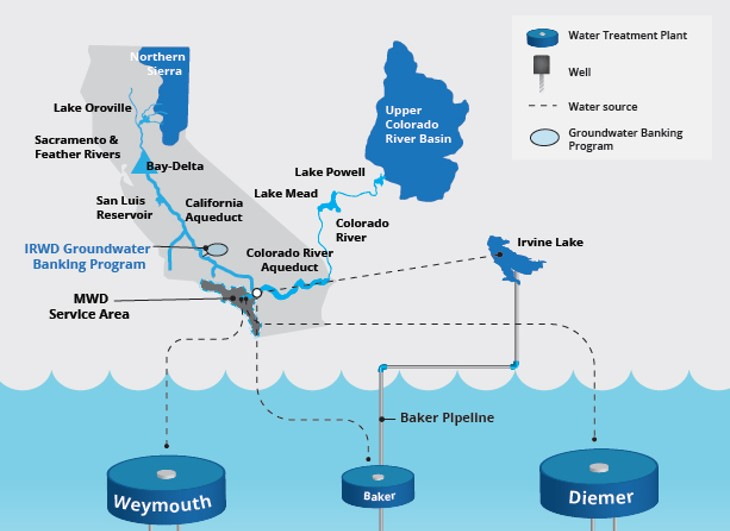
\includegraphics[scale=0.7]{Section14}\\
			      		Imhoff Cone\\
			      		\textit{Note the ml markings at the bottom of the cone}
			      		
			      		
			      	\end{center}

State Water Project (SWP).  The State Water Project conveys water from Northern California to Southern California and conveys an average of 2.8 million acre-feet per year (AFY) of water.  Sierra Nevada Mountains in Northern California receive most of the State's annual precipitation during the winter as snow to form an icepack in the mountains.  As the temperature heats up and seasons change, the icepack melts and the runoff flows into tributaries and rivers that eventually flow into a series of dams and reservoirs that finally make it to the Bay Delta.  The California Aqueduct conveys water from the Bay Delta to SoCal for treatment and use as drinking (potable) water.
Colorado River Aqueduct (CRA).  The Colorado River Aqueduct conveys water from the Colorado River to Southern California and conveys an average of 1.2 million AFY.  Similar to the SWP, the icepack and runoff from the Rocky Mountains in Colorado (and many other tributaries) are the main source of water for the Colorado River.  The Colorado River Basin supplies water to seven states (Arizona, California, Colorado, New Mexico, Nevada, Utah, and Wyoming) and Mexico.\\
\vspace{1cm}
The water quality from the SWP is generally better than the CRA.  In fact, you've probably seen (or even swam) in the SWP or CRA.  If you've driven a long distance on the I-5 freeway or visited Pyramid Lake or Castaic Lake, then you've seen the SWP.  Lake Mead, Lake Powell, Lake Havasu, and Lake Mathews are all part of the Colorado River and CRA system.  Water infrastructure is all around us!\\
\vspace{1cm}
Moving all this water requires A LOT of energy continuously for pump stations and treatment.  Roughly 20-40\% of California's total energy usage (electricity, natural gas, and diesel fuel) is used to move and treat water!  This is the "Water-Energy Nexus" whereby water usage and energy usage are so closely connected that reducing water usage and improving efficiency will not only save water resources but energy resources and cost as well!\\

\vspace{1cm}


Additional Resources:

These links provide maps that show the extent of the:

State Water Project
Colorado River Basin

To learn more about the SWP and CRA, which are considered to be engineering marvels to this day, here are a few additional references:

Department of Water Resources, State Water Project
Water Education Foundation
Maven's Notebook




Common Water Units:

1 acre = 43,560 square feet (sf).  This is about the size of an American football field. \\

Now imagine this football field being filled with 1 foot of water; this is the same as 1 acre-foot (AF).   1 AF = 325,851 gallons\\

1 million gallons (MG) = 1,000,000 gallons (gal).  It would take about two Olympic-size swimming pools to hold 1 MG of water.\\

1 million gallons per day (mgd) = 1,120 acre-feet per year (AFY)\\



\phantom{AAA}
\vspace{10cm}
\begin{center}
BLANK PAGE
\end{center}
\end{document}
